\section{Change of Basis}

\begin{frame}{Change of Basis}
	    In the standard basis, we write vectors as a linear combination of the standard basis vectors.

        \[
            \vec{x} = \mat{x_1;x_2} = x_1\mat{1;0} + x_2\mat{0;1}
        \]
        
        Likewise, we can write our \(x\) vector as a linear combination of some other basis vectors. For example, if our \(V\)-basis has basis vectors $\vec{v_1}$ and $\vec{v_2}$:
        
    \[
        \vec{x} = \tilde{x_1}\cdot\vec{v_1} + \tilde{x_2}\cdot\vec{v_2} = V\vec{\tilde{x}}
    \]
        
        We can go from the \(V\)-basis to the standard basis by applying the \(V\)-matrix to \(x\), and go from the standard basis to the \(V\)-basis by applying \(V^{-1}\).
	\end{frame}
	
	\begin{frame}{Change of Basis Diagram}
    	\begin{columns}[onlytextwidth,T]
        	\column{\dimexpr\linewidth-40mm-5mm}
        	    \begin{itemize}
        	        \item When you are doing change of basis for systems of equations, it is useful to use a diagram mapping transformations between basis
                    
                    \item Given $T$, to find $T_a$ you would trace the path from $u_a$ to $v_a$, applying each transformation to the left of the previous:
                    
                    $A \implies TA \implies A^{-1}TA$
                    
                    $T_a = A^{-1}TA$
                    
                    \item Step by step, we have $Au_a = u \implies TAu_a = v \implies A^{-1}TAu_a = v_a$
        	    \end{itemize}
    	    
    	    \column{40mm}
    	        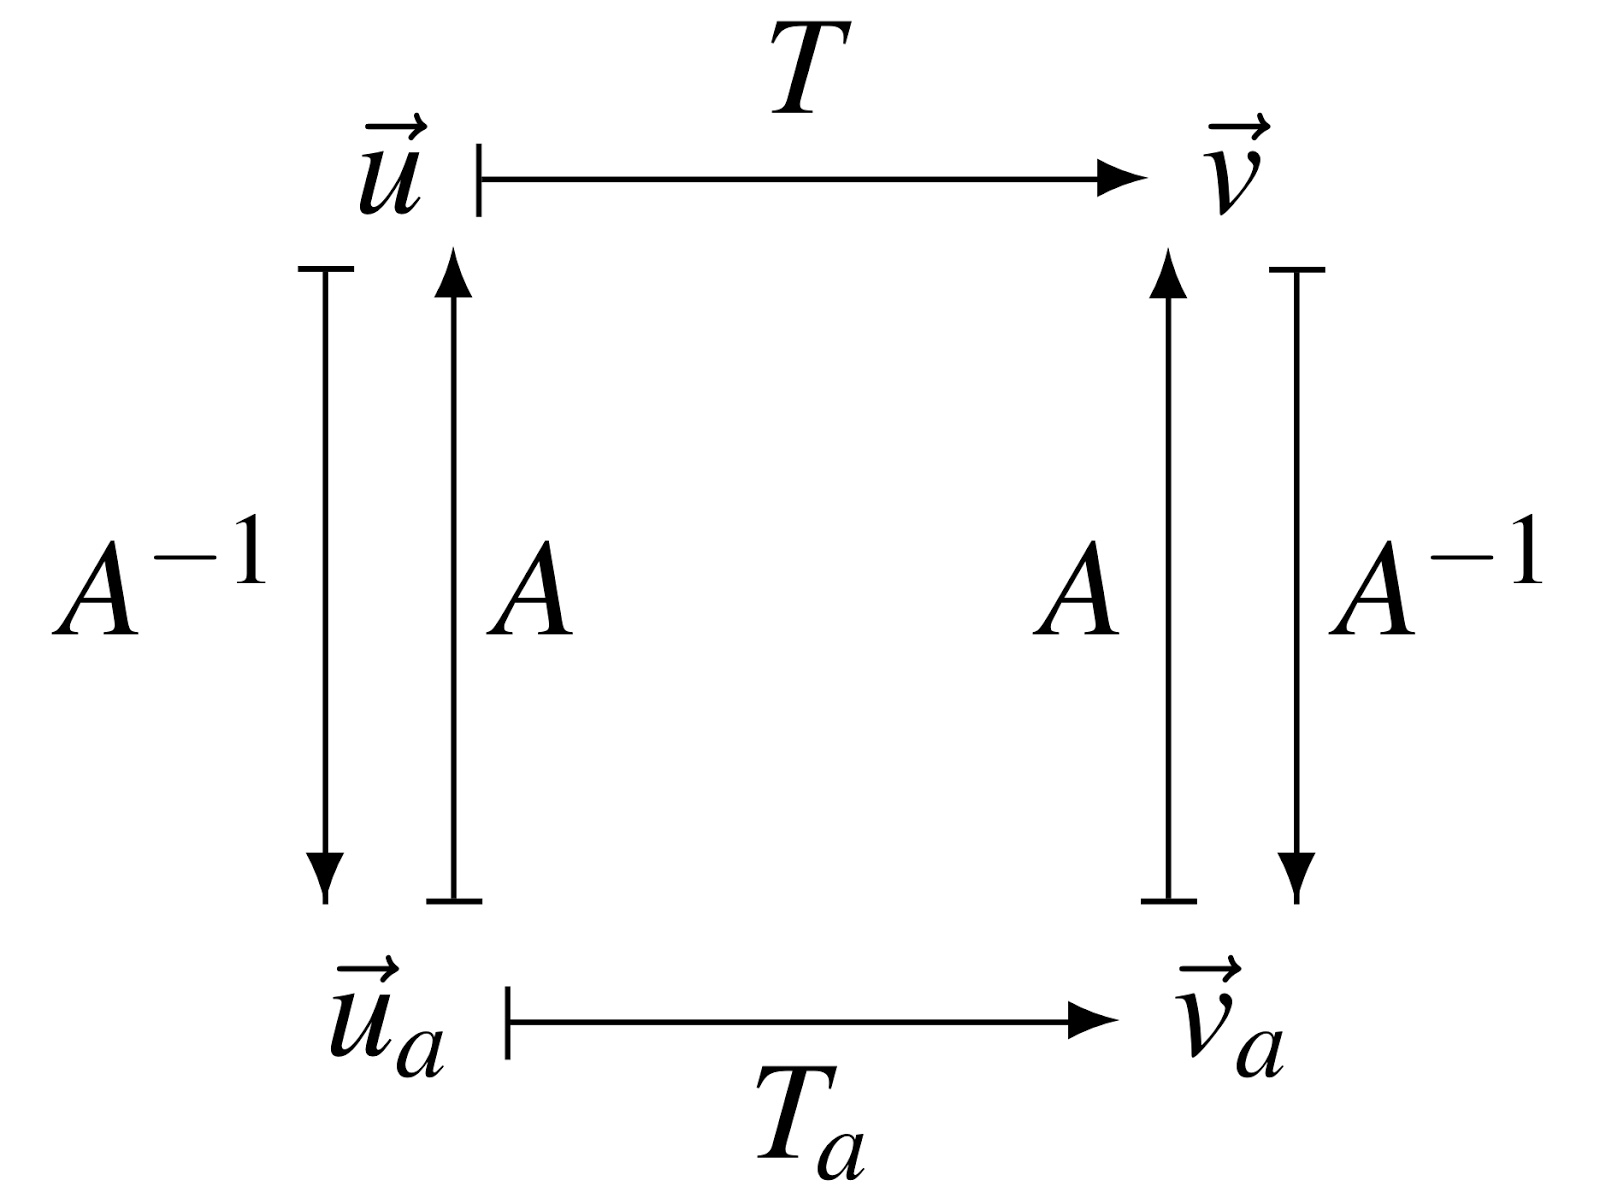
\includegraphics[width=40mm]{./images/change-of-basis-diagram.jpeg}
	    \end{columns}
	\end{frame}
	
